\documentclass{article}
\usepackage{graphicx} % Required for inserting images

\usepackage{auto-pst-pdf} % Enable PSTricks with pdflatex
% If using Overleaf, the -shell-escape flag is already enabled by default for auto-pst-pdf to work
\usepackage{pst-eucl} % Euclidean geometry

\usepackage{tikz} % ChatGPT likes this for drawing some things
\usetikzlibrary{calc,intersections}

\usepackage{mathtools}


\title{MAT 357-557 Numerical Analysis Project 2}
\author{Austin Zhu, Brillan Morgan, Osprey Varboncoeur}
\date{Spring 2024}

\begin{document}

\maketitle

\section{The Idea}
\label{sec:the_idea}
Our goal is to use a set of points to generate an aesthetically pleasing curve consisting only of circle arcs and line segments. Our method interpolates between points by interpreting pairs of points as defining circles, then drawing arcs of those circles and connecting those arcs with line segments at tangent points.

\subsection{Interpreting the Input Data Set}
For an input data set of \( n \) points, let the \( \frac{n}{2} \) pairs of points be:

\[ P_0, P_1, \ldots, P_{n-2}, P_{n-1} \]

Note that \( n \) must be an even number. Let the even-indexed points be the "Control" points, the center points of the circles:

\[ P_0 = C_0, P_2 = C_1, \ldots, P_{n-2} = C_{\frac{n}{2}-1} \]

Let the odd-indexed points be the "Anchor" points, the points on the circumference of the circles:

\[ P_1 = A_0, P_3 = A_1, \ldots, P_{n-1} = A_{\frac{n}{2}-1} \]

%\vspace{0.2cm} % Adjust the vertical space as needed

\begin{figure}
\centering
\begin{tikzpicture}
    % Draw the circle
    \draw (0,0) circle (2cm);

    % Label the center
    \draw (0,0) node[circle,fill,inner sep=1.5pt,label=below:$C_i$] {};

    % Draw a point on the circumference
    \draw (135:2cm) node[circle,fill,inner sep=1.5pt,label=above left:$A_i$] {};
\end{tikzpicture}
\caption{Pairs of points in from the input data set represent a circle.}
\label{fig:pairs_of_points_define_a_circle}
\end{figure}

%\vspace{0.2cm} % Adjust the vertical space as needed

Each pair of points \( \{C_i, A_i\} \) define a circle, as shown in Fig. \ref{fig:pairs_of_points_define_a_circle}. The \( \frac{n}{2} \) pairs of points define \( \frac{n}{2} \) circles. A minimum of four points defining two circles (\( n \geq 4 \)) is required to use our method.

\subsubsection{Adjacency}
Circles that are adjacent \textit{in the input data list} must be disjoint, that is, they must not intersect or be one inside the other. Circle \( \{C_i, A_i\} \) must be disjoint from circle \( \{C_{i-1}, A_{i-1}\} \), and also disjoint from circle \( \{C_{i+1}, A_{i+1}\} \). Circle \( \{C_i, A_i\} \) may or may not be disjoint from any other circle in the input data set. Note that there are only disjoint-ness requirements for circles based on their positions in the input data set, not based on any geometric relationship between them.


\subsection{A Parametric, Piecewise Curve}
\label{subsec:definition_of_curve}
Let the final curve be defined by a parametric piecewise function of $t$:
\begin{equation}
    \label{eq:O(t)}
\overrightarrow{O}(t) = \overrightarrow{O}_{\lfloor t \rfloor}(t - \lfloor t \rfloor) = \begin{cases}
S_0(t) & \text{for } 0 \leq t < 1, \\
L_1(t - 1) & \text{for } 1 \leq t < 2, \\
R_2(t - 2) & \text{for } 2 \leq t < 3, \\
S_3(t - 3) & \text{for } 3 \leq t < 4, \\
L_4(t - 4) & \text{for } 4 \leq t < 5, \\
R_5(t - 5) & \text{for } 5 \leq t < 6, \\
\vdots & \\
S_{\frac{3n}{2}-6}(t - \frac{3n}{2}-6) & \text{for } \frac{3n}{2}-6 \leq t < \frac{3n}{2}-5, \\
L_{\frac{3n}{2}-5}(t - \frac{3n}{2}-5) & \text{for } \frac{3n}{2}-5 \leq t < \frac{3n}{2}-4, \\
R_{\frac{3n}{2}-4}(t - \frac{3n}{2}-4) & \text{for } \frac{3n}{2}-4 \leq t < \frac{3n}{2}-3, \\
A_{\frac{n}{2}-1} & \text{for } t = \frac{3n}{2}-3
\end{cases}
\end{equation}

Where:
\begin{itemize}
    \item $n$ is the number of points in the input data set
    \item $\lfloor \cdot \rfloor$ is the floor function, which rounds down to the largest integer value less than or equal to the variable inside. Examples: $\lfloor 2.0 \rfloor = 2.0$, $\lfloor 2.6 \rfloor = 2.0$.
    \item The initial direction of arc travel around circle $\{C_0, A_0\}$ starting from $A_0$ is defined to be counter-clockwise.
    \item $S$ is the "Sender" function that gives the portion of the $\{C_i, A_i\}$ circle's arc which connects its Anchor point $A_i$ to its tangent "sending" point $T_{iS}$. The sending point is the point on the circle tangent to the line segment\footnote{For any two disjoint circles, there exist four tangent lines: two internal tangent lines and two external tangent lines (see Fig. \ref{fig:external_tangents_only}). For our curve, we will consider only external tangent lines.} connecting circle $\{C_i, A_i\}$ to circle $\{C_{i+1}, A_{i+1}\}$ such that the resulting curve has no corner, as seen in Fig. \ref{fig:does_not_create_a_corner}.
    Note that the counter-clockwise direction of arc travel determines which of the tangent points on circle $\{C_i, A_i\}$ will be the correct tangent sending point $T_{iS}$, that is, the one that does not create a corner. Note also that defining the travel direction for the first sending arc to be counter-clockwise also defines travel direction for all arcs in the curve to be counter-clockwise.
    \item $L$ is the "Line" function that gives the line segment connecting the tangent sending point $T_{iS}$ on circle $\{C_i, A_i\}$ to the tangent receiving point $T_{iR}$ on circle $\{C_{i+1}, A_{i+1}\}$.
    \item $R$ is the "Receiver" function that gives the portion of the $\{C_{i+1}, A_{i+1}\}$ circle's arc that connects the tangent receiving point $T_{iR}$ to its Anchor point $A_{i+1}$.
\end{itemize}

\begin{figure}
    \centering
    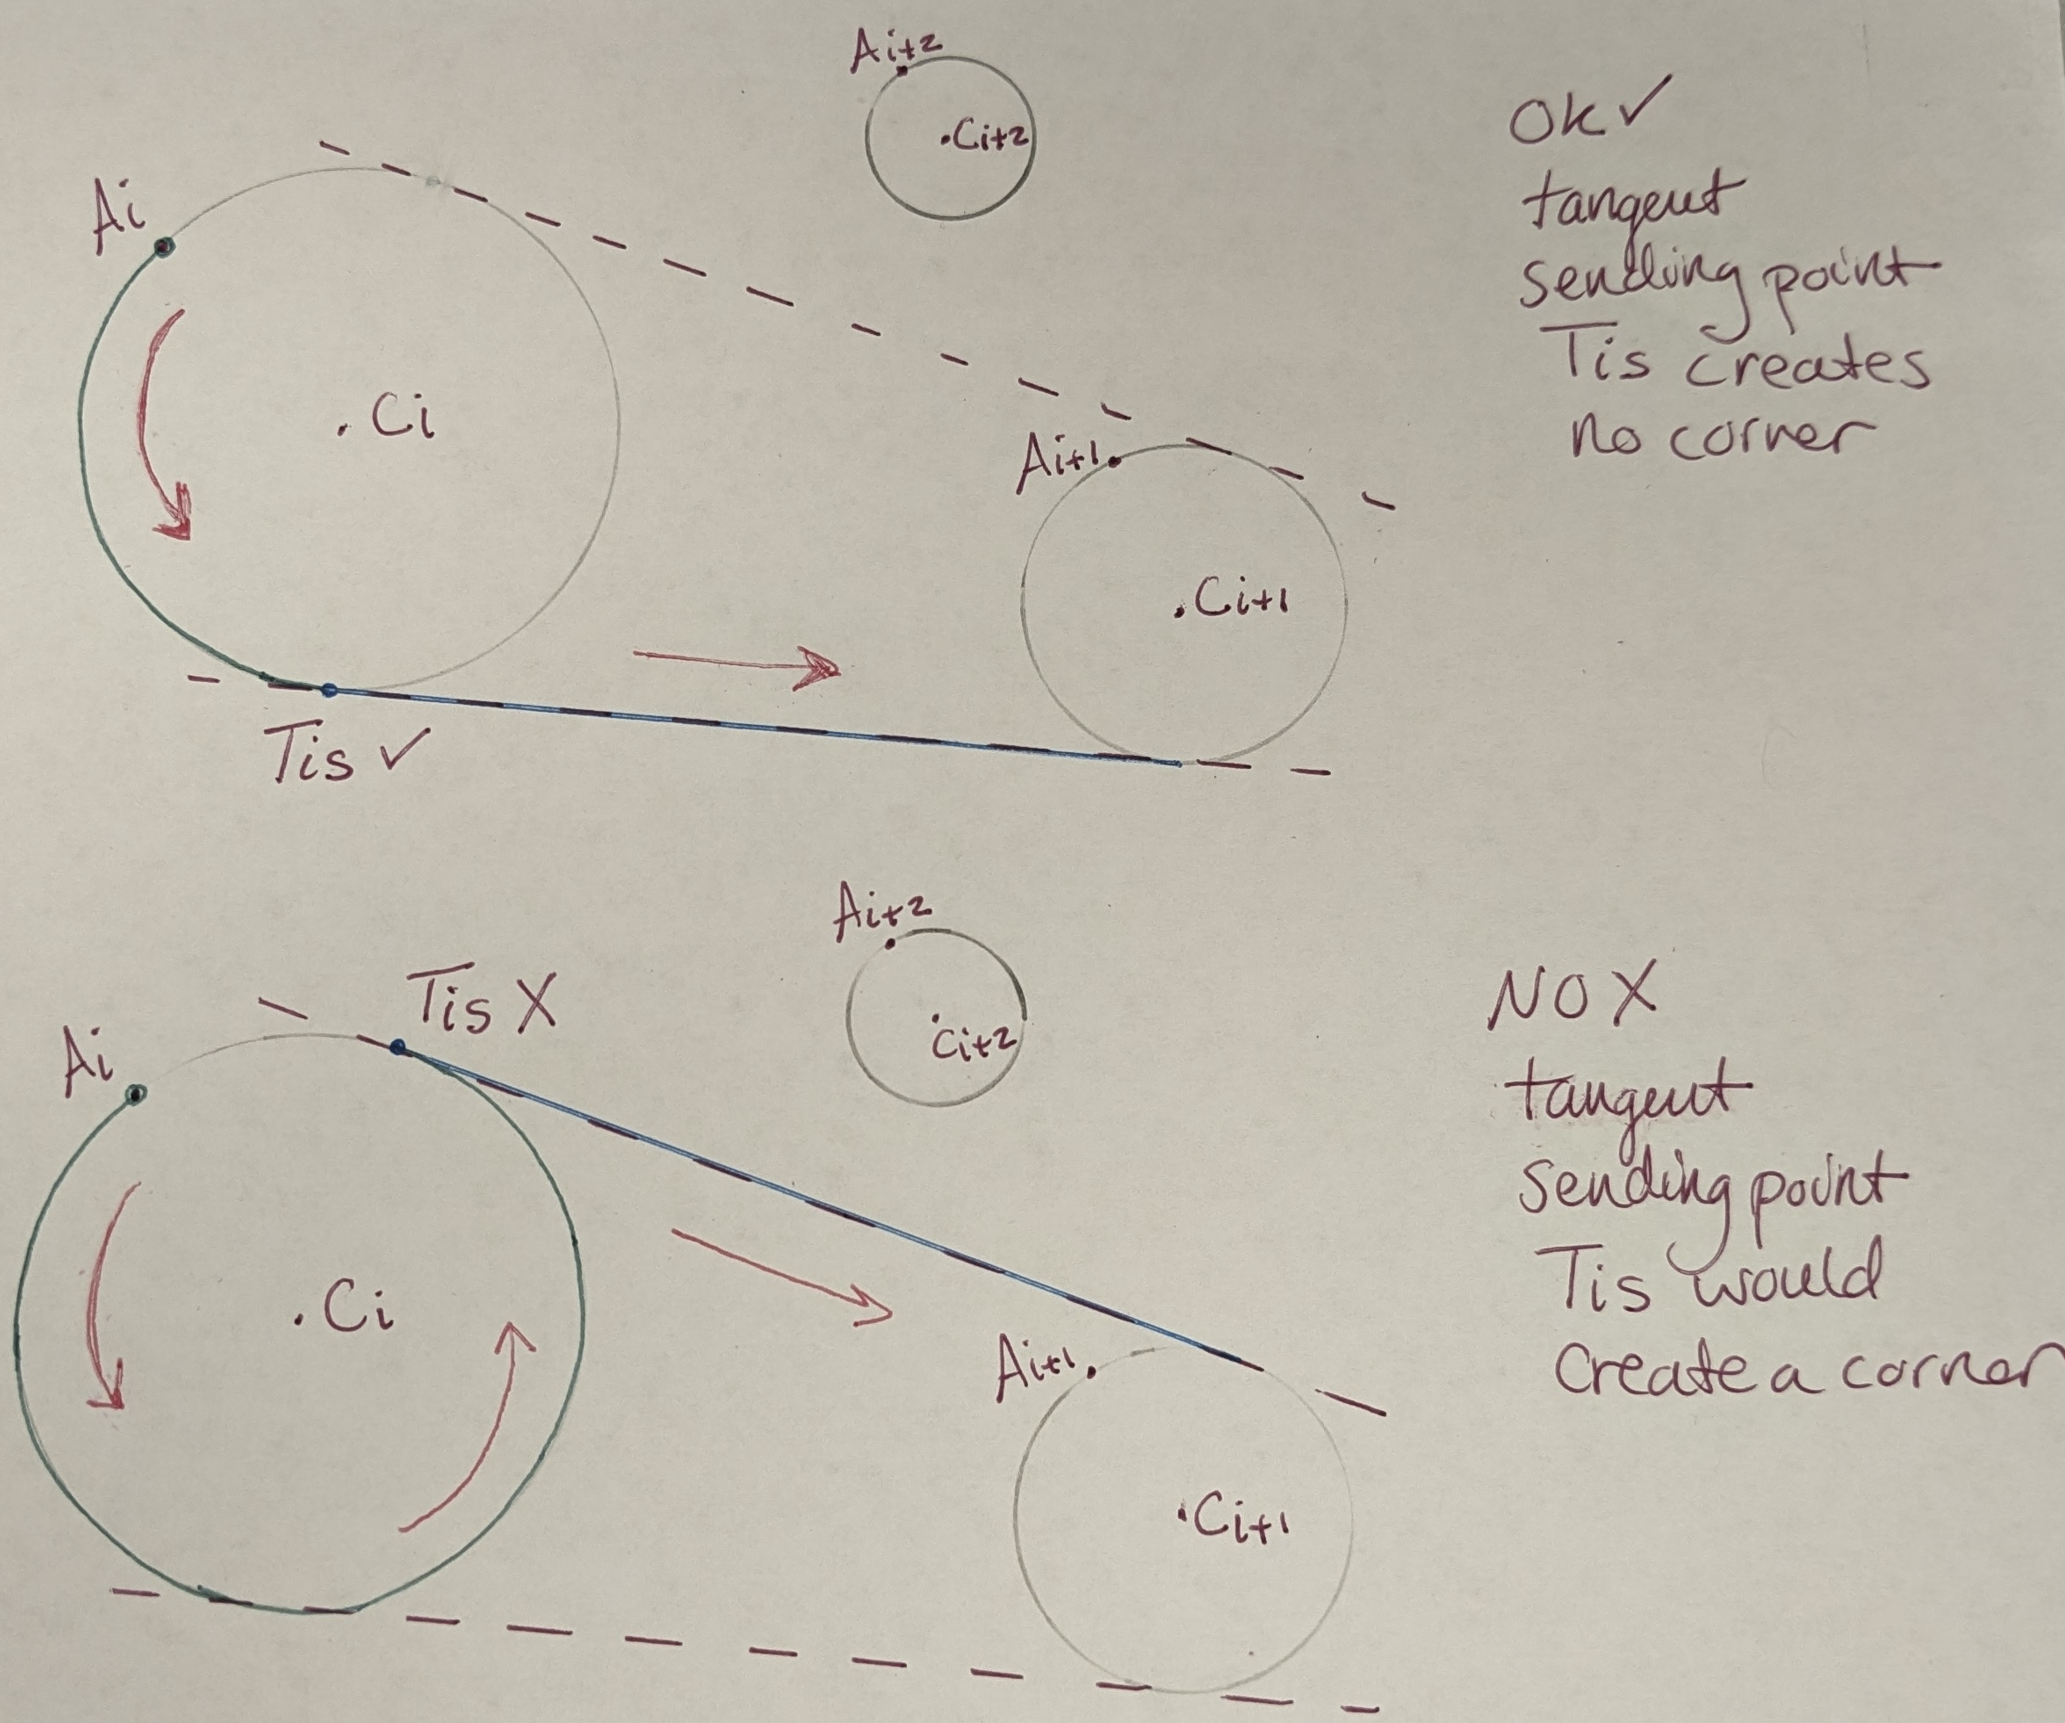
\includegraphics[width=1.0\textwidth]{NoCorner.png}
    \caption{The correct tangent sending point $T_{iS}$ is the one that does not create a corner.}
    \label{fig:does_not_create_a_corner}
\end{figure}

Fig. \ref{fig:SLRExample} shows an example resulting curve with the $S$ "Sending" function plots shown in green, the $L$ "Line" plots shown in blue, and the $R$ "Receiver" plots shown in orange.
\begin{figure}
    \centering
    \includegraphics[width=1.0\textwidth]{FigureXExampleOfSLR_Cropped.png}
    \caption{Example curve showing $S$ "Sending" function plots (green), $L$ "Line" plots (blue), and $R$ "Receiver" plots (orange)}
    \label{fig:SLRExample}
\end{figure}

\begin{figure}[htbp]
    \centering
    %\vspace{0.2cm} % Adjust the vertical space as needed
    \begin{tikzpicture}
        % Draw the larger circle
        \draw (0,0) circle (2cm);
        % Draw the smaller circle
        \draw (5,0) circle (1cm);


        % Tangency points on the larger circle (for reference)
        \coordinate (T1) at (0.4, 1.96);
        \coordinate (T2) at (0.4, -1.96);

        % Tangency points on the smaller circle (for reference)
        \coordinate (T3) at (5.2, 0.98);
        \coordinate (T4) at (5.2, -0.98);

        % Draw the tangent lines (for reference)
        \draw[blue] (T1) -- (T3);
        \draw[blue] (T2) -- (T4);

        % Internal tangency points
        \coordinate (T5) at (1.2, 1.6);
        \coordinate (T6) at (1.2, -1.6);
        \coordinate (T7) at (4.4, 0.8);
        \coordinate (T8) at (4.4, -0.8);

        % Draw the internal tangent lines in red
        \draw[red] (T5) -- (T8);
        \draw[red] (T6) -- (T7);
    \end{tikzpicture}
    \caption{The tangent lines of two disjoint circles: two internal tangent lines (red) and two external tangent lines (blue). Our curve considers only external tangent lines.}
    \label{fig:external_tangents_only}
\end{figure}
%\vspace{0.2cm} % Adjust the vertical space as needed
\subsubsection{Interpretation and Usage of Parameter Variable $t$}
The range of values that can be used with $\overrightarrow{O}(t)$ is $0 \leq t \leq \frac{3n}{2}$. The first point of the curve $P_1 = A_0$ is plotted by function $S_0$ when $t = 0$. The final point of the curve $P_{n-1} = A_{\frac{n}{2}-1}$ is plotted directly when $t = \frac{3n}{2}$, without using any of the $SLR$ functions.
Table \ref{tab:n_t_and_SLR_relationship} gives examples showing the relationship between $n$, the maximum value of $t$, and the indices of all $SLR$ functions (and the final $A$ point) of the piecewise curve definition.

\begin{table}[htbp]
    \centering
    \begin{tabular}{|c|c|c|c|}
        \hline
        Input data count & \multicolumn{1}{c|}{\begin{tabular}[t]{@{}c@{}}
            $n = 4$ points \\
            $\frac{n}{2} = 2$ circles
        \end{tabular}} &
        \multicolumn{1}{c|}{\begin{tabular}[t]{@{}c@{}}
            $n = 6$ points \\
            $\frac{n}{2} = 3$ circles
        \end{tabular}} &
        \multicolumn{1}{c|}{\begin{tabular}[t]{@{}c@{}}
            $n = 8$ points \\
            $\frac{n}{2} = 4$ circles
        \end{tabular}} \\
        \hline
        All piecewise functions & \multicolumn{1}{|c|}{\begin{tabular}[t]{@{}c@{}}
            $S_0$ \\
            $L_1$ \\
            $R_2$ \\
            $A_1$
        \end{tabular}} &
        \multicolumn{1}{|c|}{\begin{tabular}[t]{@{}c@{}}
            $S_0$ \\
            $L_1$ \\
            $R_2$ \\
            $S_3$ \\
            $L_4$ \\
            $R_5$ \\
            $A_2$
        \end{tabular}} &
        \multicolumn{1}{|c|}{\begin{tabular}[t]{@{}c@{}}
            $S_0$ \\
            $L_1$ \\
            $R_2$ \\
            $S_3$ \\
            $L_4$ \\
            $R_5$ \\
            $S_6$ \\
            $L_7$ \\
            $R_8$ \\
            $A_3$
        \end{tabular}} \\
        \hline
        Range of possible $t$ values & \multicolumn{1}{|c|}{\begin{tabular}[t]{@{}c@{}}
            $0 \leq t \leq \frac{3n}{2}-3$ \\
            \hspace{1.5em}$\leq \frac{3 \cdot 4}{2}-3$ \\
            $0 \leq t \leq 3$
        \end{tabular}} &
        \multicolumn{1}{|c|}{\begin{tabular}[t]{@{}c@{}}
            $0 \leq t \leq \frac{3n}{2}-3$ \\
            \hspace{1.5em}$\leq \frac{3 \cdot 6}{2}-3$ \\
            $0 \leq t \leq 6$
        \end{tabular}} &
        \multicolumn{1}{|c|}{\begin{tabular}[t]{@{}c@{}}
            $0 \leq t \leq \frac{3n}{2}-3$ \\
            \hspace{1.5em}$\leq \frac{3 \cdot 8}{2}-3$ \\
            $0 \leq t \leq 9$
        \end{tabular}} \\
        \hline
    \end{tabular}
    \caption{2x4 table with specified content}
    \label{tab:n_t_and_SLR_relationship}
\end{table}

\subsubsection{Overlapping Arcs}
Consider the scenario where the position of Anchor point $A_{i+1}$ on circle $\{C_{i+1}, A_{i+1}\}$ causes the receiving arc (going from $T_{iR}$ to $A_{i+1}$) to overlap with the sending arc (going from $A_{i+1}$ to $T_{(i+1)S}$). In this scenario, the entire $\{C_{i+1}, A_{i+1}\}$ circle will be plotted. Further, some of circle $\{C_{i+1}, A_{i+1}\}$ will be plotted twice: first by the $R$ function, then again by the $S$ function.\\ \\
\textbf{DIAGRAM TODO}\\ \\
Such overlapping of receiving and sending arcs does not affect which tangent point will become the $T_{(i+1)S}$ tangent sending point for circle $\{C_{i+1}, A_{i+1}\}$. The correct tangent sending point is determined only by the direction of arc travel, which is defined to start as counterclockwise and guaranteed to remain counterclockwise for all arcs in the curve.

\section{The Computation}
\label{sec:the_computation}
The computation of $SLR$ functions that are adjacent in the piecewise definition of $\overrightarrow{O}(t)$ are closely related, so we will discuss them as a group. Further, the computation of an $SLR$ group uses \textit{only} four points from the input data set: the two that define the circle of the sending arc and the two that define the circle of the receiving arc. No results from computation of other $SLR$ groups are required.

\subsection{Naming Conventions and Name Conversion}
\textbf{SUBSECTION INTRO TO AVOID STACKED HEADINGS}
\subsubsection{Conversion of $SLR$ Function Subscripts to Circle Indices}
\label{subsubsec:SLR_subscript_conversion}
During the computation, we will use the subscript of the called $SLR$ function to look up the corresponding points of the sending circle $\{C_i, A_i\}$ and the points of the receiving circle $\{C_{i+1}, A_{i+1}\}$. The conversion from $SLR$ function subscripts to circle indices is shown in Table \ref{tab:my_conversion_from_SLR_subscript_to_circle_subscripts}, with an example conversion worked out in Table \ref{tab:my_conversion_from_SLR_subscript_to_circle_subscripts_EXAMPLE}.

Note that all three functions in an $SLR$ group share the same $\{C_i, A_i\}$ circle for the sending arc and the same $\{C_{i+1}, A_{i+1}\}$ circle for the receiving arc.

The complexity of this process serves to ensure that the range of $t$ values passed to any $SLR$ function is $0 \leq t < 1$. To make that happen, we define the subscript of the first $S$ function to be $0$ and for the subscript of each following $SLR$ piecewise function to be one greater that the subscript of the one immediately prior.

\begin{table}[h]
\centering
\begin{tabular}{|c|c|c|}
\hline
$\text{SLR Function Called}$ & $\text{Circle of Sending Arc}$ & $\text{Circle of Receiving Arc}$ \\
\hline
$S_u$ & $\{C_\frac{u}{3}, A_\frac{u}{3}\}$ & $\{C_\frac{u}{3}, A_\frac{u}{3}\}$\\
$L_v$ & $\{C_\frac{v-1}{3}, A_\frac{v-1}{3}\}$ & $\{C_\frac{v+2}{3}, A_\frac{v+2}{3}\}$\\
$R_w$ & $\{C_\frac{w-2}{3}, A_\frac{w-2}{3}\}$ & $\{C_\frac{w+1}{3}, A_\frac{w+1}{3}\}$\\
\hline
\end{tabular}
\caption{A simple table}
\label{tab:my_conversion_from_SLR_subscript_to_circle_subscripts}
\end{table}

\begin{table}[h]
\centering
\begin{tabular}{|c|c|c|}
\hline
$\text{SLR Function Called}$ & $\text{Circle of Sending Arc}$ & $\text{Circle of Receiving Arc}$ \\
\hline
$S_6$ & $\{C_\frac{6}{3}, A_\frac{6}{3}\} = \{C_2, A_2\}$ & $\{C_\frac{6+3}{3}, A_\frac{6+3}{3}\} = \{C_3, A_3\}$\\
$L_7$ & $\{C_\frac{7-1}{3}, A_\frac{7-1}{3}\} = \{C_2, A_2\}$ & $\{C_\frac{7+2}{3}, A_\frac{7+2}{3}\} = \{C_3, A_3\}$\\
$R_8$ & $\{C_\frac{8-2}{3}, A_\frac{8-2}{3}\} = \{C_2, A_2\}$ & $\{C_\frac{8+1}{3}, A_\frac{8+1}{3}\} = \{C_3, A_3\}$\\
\hline
\end{tabular}
\caption{A simple table}
\label{tab:my_conversion_from_SLR_subscript_to_circle_subscripts_EXAMPLE}
\end{table}

\subsubsection{Symbols and Names Local to $SLR$ Group Computation}
\label{subsub:local_point_indices}
Since an $SLR$ group can be computed in complete isolation, local to its computation we will refer to the sending circle as $\{C_1, A_1\}$ and the receiving circle as $\{C_2, A_2\}$. Within this context, the $\{C_1, A_1\}$ and $\{C_2, A_2\}$ names effectively "shadow" the meaning of those names outside of the local context. The authors have lots of work expressed in this local naming scheme, and have opted to continue use of it here for sanity purposes.

The computation of an $SLR$ group will never refer to any points other than those defining its sending circle and receiving circle. The conversion from sub-subsection \ref{subsubsec:SLR_subscript_conversion} is the only connection between the computation of an $SLR$ group and any names from the input data set.

Within the context of computing a given $SLR$ group, after the indices of the circles have been converted, we will refer to the $SLR$ functions without any subscript, as the purpose of the subscript is to facilitate identifying the indices of the points on which to operate.

Further, local to $SLR$ group computation, the parameter $t$ passed into an $SLR$ function will be the result of the $t - \lfloor t \rfloor$ step computed during the lookup (as shown in the piecewise function definition of $\overrightarrow{O}(t)$ in subsection \ref{subsec:definition_of_curve}).

\subsection{Computation of an $SLR$ Function Group}
\label{subsec:SLR_group_computation}
Section \ref{sec:the_idea} described \textit{what} our method does as a whole: it gives the piecewise parametric function $\overrightarrow{O}(t)$ which plots the curve represented by the $\frac{n}{2}$ pairs of input points, supporting values $0 \leq t \leq \frac{3n}{2}-3$.

This section details the computation of the $S$, $L$ and $R$ functions and substantiates their logic with principles from geometry and trigonometry.

\subsubsection{The Sending Function $S$}
\label{subsubsec:sending_function_S}
The sending function $S$ gives an arc on circle $\{C_1, A_1\}$ starting from known Anchor point $A_1$ and ending at tangent "sending" point $T_{1S}$. For the correct external tangent line between circle $\{C_1, A_1\}$ and circle $\{C_2, A_2\}$, $T_{1S}$ is the tangent point that of that line to circle $\{C_1, A_1\}$. We must find an expression for $T_{1S}$. To that end, we construct a diagram of geometric relationships between circle $\{C_1, A_1\}$ and circle $\{C_2, A_2\}$ (see Figure X).

\paragraph{Finding an expression for $T_{1S}$}
We draw the external tangent lines to the circles, and draw a line segment connecting circle center $C_1$ to tangent point $T_{1S}$. We note that the length of this line segment is equal to the radius of circle $\{C_1, A_1\}$. Let $r_1$ be this radius length:

\begin{equation}
    \label{eq:r_1}
    r_1 = \sqrt{(A_1.x - C_1.x)^2 + (A_1.y - C_1.y)^2}
\end{equation}

We also note that the angle between the radius line segment and the tangent line is a right angle.

We draw a line segment connecting circle center $C_2$ to tangent point $T_{1R}$. We note that the length of this line segment is equal to the radius of circle $\{C_2, A_2\}$. Let $r_2$ be this radius length:

\begin{equation}
    \label{eq:r_2}
r_2 = \sqrt{(A_2.x - C_2.x)^2 + (A_2.y - C_2.y)^2}
\end{equation}

We draw a line segment connecting circle center $C_1$ to circle center $C_2$. We note that the length of this line segment is equal to the distance between the centers of the circles. Let $d$ be this distance:

\begin{equation}
    \label{eq:d}
    d = \sqrt{(C_2.x - C_1.x)^2 + (C_2.y - C_1.y)^2}
\end{equation}

For the line segment connecting $C_1$ to $C_2$, we draw a line segment parallel to it from $T_{1R}$ towards circle $\{C_1, A_1\}$. The line segment is of length $d$ and ends at a point on the radius line segment between $C_1$ and $T_{1S}$. Let this point be point $Q$.

We note that the angle between the $C_1$, $T_{1S}$ line segment and the line connecting $C_1$, $C_2$ is equal to the angle between the $Q$, $T_{1S}$ line segment and the $Q$, $T_{1R}$ line segment. Let that angle be $\theta$.

We note that the length of the $Q$, $T_{1S}$ line segment is equal to $r_1 - r_2$.

We observe that we have found a right triangle where the hypotenuse is the $Q$, $T_{1S}$ line segment, the adjacent side to $\theta$ is the $Q$, $T_{1S}$ line segment, and the opposite side to $\theta$ is the $T_{1S}$,  $T_{1R}$ line segment. Using the Pythagorean theorem, we can form an expression for $\theta$:

\begin{equation}
    \label{eq:theta}
    \theta = \arccos\left(\frac{r_1 - r_2}{d}\right)
\end{equation}

We observe that point $T_{1S}$ is at angle $-\theta$ from the $C_1$, $C_2$ line segment. We note that in general, the $C_1$, $C_2$ line segment will not be aligned with the $x$ axis. Let $\alpha$ be the angle between the $C_1$, $C_2$ line segment and the $x$ axis:

\begin{equation}
    \label{eq:alpha}
    \alpha = atan2(C_2.y - C_1.y, C_2.x - C_1.x)
\end{equation}

Where $atan2$ is the the two-argument arctangent function that returns the angle in the appropriate quadrant, taking into account the signs of both x and y.

Finally we can express $T_{1S}$ in terms of all known quantities:

\begin{equation}
    \label{eq:T_1S.x}
    T_{1S}.x = C_1.x + r_1 * cos(\alpha - \theta)
\end{equation}

\begin{equation}
    \label{eq:T_1S.y}
    T_{1S}.y = C_1.y + r_1 * sin(\alpha - \theta)
\end{equation}

That is, $T_{1S}$ is distance $r_1$ from $C_1$ at angle $-\theta$, where $\alpha$ is the angle between the $C_1$, $C_2$ line segment and the $x$ axis.

\paragraph{Converting from Parameter $t$ to an Angle}
Recall that the purpose of the $S$ function is to draw the arc from $A_1$ to $T_{1S}$. Specifically, the $S(t)$ gives the point on that arc which corresponds to the parameter $t$, where $0 \leq t < 1$. $t = 0$ corresponds to $A_1$, while $t = 1$ would correspond to $T_{1S}$.\footnote{The $S$ function operates on $0 \leq t < 1$, so it doesn't draw $T_{1S}$, rather, the $L$ function will.}

To do that interpolation, we need both $A_1$ and $T_{1S}$ expressed as angles.\footnote{Why bother to express $T_{1S}$ as $(x,y)$ coordinates in the first place? They will be useful when we get to discussing the $L$ function.} Let $\omega_{A1}$ be the angle of $A_1$ and let $\omega_{T1S}$ be the angle of $T_{1S}$:

\begin{equation}
    \label{eq:omega_A1}
    \omega_{A1} = atan2(A_1.y - C_1.y, A_1.x - C_1.x)
\end{equation}

\begin{equation}
    \label{eq:omega_T1S}
    \omega_{T1S} = atan2(T_{1s}.y - C_1.y, T_{1s}.x - C_1.x)
\end{equation}

Finally, let $\Theta_S(t)$ be a function that gives the interpolated angle between $A_1$ and $T_{1S}$ for any $0 \leq t < 1$:

\begin{equation}
    \label{eq:Theta_S(t)}
    \Theta_S(t) = (1-t) \omega_{A1} + t \omega_{T1S}
\end{equation}

\paragraph{Bringing it All Together: Sending Function $S$}
Now that we can convert directly from parameter $t$ to the corresponding angle on the sending arc, we can use that result to construct the $S$ piecewise function itself:

\begin{equation}
    \label{eq:S(t)}
    S(t) = C_1 + r_1 * (cos( \Theta_S(t) ), sin( \Theta_S(t) ))
\end{equation}

That is, for a given $t$, we plot the point that is distance $r_1$ from point $C_1$ at the interpolated angle that corresponds to parameter $t$.


\subsubsection{The Line Segment Function $L$}
\label{subsubsec:line_segment_function_L}
The "Line" function $L$ gives the line segment connecting the tangent sending point $T_{1S}$ on circle $\{C_1, A_1\}$ to the tangent receiving point $T_{2R}$ on circle $\{C_2, A_2\}$.

The $L$ function gives the point on the line that corresponds to parameter $t$, where $0 \leq t < 1$. $t = 0$ corresponds to $T_{1S}$, while $t = 1$ would correspond to $T_{1R}$.\footnote{The $L$ function operates on $0 \leq t < 1$, so it doesn't draw $T_{1R}$, rather, the $R$ function will.}

To do this interpolation, we need $T_{1S}$ and $T_{1R}$ expressed as $(x,y)$ coordinates. We already have $T_{1S}$ from sub-subsection \ref{subsubsec:sending_function_S}. Following the same logic and Using the same $\alpha$ and $\theta$, we can express $T_{1R}$ in terms of all known quantities:

\begin{equation}
    \label{eq:T_1R.x}
    T_{1R}.x = C_2.x + r_2 * cos(\alpha - \theta)
\end{equation}

\begin{equation}
    \label{eq:T_1R.y}
    T_{1R}.y = C_2.y + r_2 * sin(\alpha - \theta)
\end{equation}

Now that we have the starting point of the line segment $T_{1S}$ and the ending point of the line segment $T_{1R}$, we can construct the $L$ piecewise function itself:

\begin{equation}
    \label{eq:L(t)}
    L(t) = T_{1S} + t * ( T_{1R} - T_{1S} )
\end{equation}

Thinking of $T_{1R} - T_{1S}$ as a vector from $T_{1S}$ to $T_{1R}$, $L(t)$ gives the point that is offset from the starting point $T_{1S}$ in the direction of $T_{1R} - T_{1S}$, scaled by $t$.

\subsubsection{The Receiving Function $R$}
The receiving function $R$ gives an arc on circle $\{C_2, A_2\}$ starting from tangent "receiving" point $T_{1R}$ and ending at known Anchor point $A_2$. For the correct external tangent line between circle $\{C_1, A_1\}$ and circle $\{C_2, A_2\}$, $T_{1R}$ is the tangent point of the line to circle $\{C_2, A_2\}$.

Specifically, $R(t)$ gives the point on that arc which corresponds to the parameter $t$, where $0 \leq t < 1$. $t = 0$ corresponds to $T_{1R}$, while $t = 1$ would correspond to $A_{2}$.\footnote{The $R$ function operates on $0 \leq t < 1$, so it doesn't draw $A_2$. The final point of the curve is plotted directly by the piecewise definition of $\overrightarrow{O}(t)$ without using any of the $SLR$ functions. }

We already have $T_{1R}$ from sub-subsection \ref{subsubsec:line_segment_function_L}, and $A_2$ is given. We need to express both $T_{1R}$ and $A_2$ as angles. Let $\omega_{T1R}$ be the angle of $T_{1R}$ and $\omega_{A2}$ be the angle of $A_2$:

\begin{equation}
    \label{eq:omega_T1R}
    \omega_{T1R} = atan2(T_{1R}.y - C_2.y, T_{1R}.x - C_2.x)
\end{equation}

\begin{equation}
    \label{eq:omega_A2}
    \omega_{A2} = atan2(A_2.y - C_2.y, A_2.x - C_2.x)
\end{equation}

Finally, let $\Theta_R(t)$ be a function that gives the interpolated angle between $T_{1R}$ and $A_2$ for any $0 \leq t < 1$:

\begin{equation}
    \label{eq:Theta_R(t)}
    \Theta_R(t) = (1-t) \omega_{T1R} + t \omega_{A2}
\end{equation}

Now that we can convert directly from parameter $t$ to the corresponding angle on the sending arc, we can use that result to construct the $R$ piecewise function itself:

\begin{equation}
    \label{eq:R(t)}
    R(t) = C_2 + r_2 * (cos( \Theta_R(t) ), sin( \Theta_R(t) ))
\end{equation}

That is, for a given $t$, we plot the point that is distance $r_2$ from point $C_2$ at the interpolated angle that corresponds to parameter $t$.


\subsubsection{Plotting the Final Point $A_{\frac{n}{2}-1}$}
Outside the scope of any $SLR$ function, the final point of the curve $P_{n-1} = A_{\frac{n}{2}-1}$ is plotted directly by the piecewise definition of $\overrightarrow{O}$ when $t = \frac{3n}{2}$. Note that this is the same point that final $R$ function did not plot because $t$ never reached $1$ inside its context.

\section{Notable Curve Properties}
Our curve connects only the Anchor points from the input data set, that is, the points on the edges of the circles. The Control points serve only to define the center point of each circle. Thus, we have borrowed the point naming convention  of B\'ezier curves.

Our curve has no discontinuities or corners. It consists of only circle arcs connected by line segments at mutual tangent points. Since our curve is parametric and not a function of x, it can cross back across where it has already been on the x axis. Fulfilling our primary goal, a very nice property of our curve is that it flows pleasingly along its path even though it is made up entirely of simple geometric constructs: circle arcs and line segments.

Our method is axis-agnostic, that is, \\
\textbf{SHOW EXAMPLE OF AXIS-AGNOSTICISM}\\

As we discussed at the start of section \ref{sec:the_computation}, the computation of an $SLR$ group does not require information from the computation of any other $SLR$ group (e.g., derivatives). This is one significant advantage that our method has over interpolation methods such as Lagrange interpolation and splines: each $SLR$ group can be computed in isolation, there is no huge system of equations required to represent the curve as a whole.




\section{Further Ideas}
What else we wanted to try
What else we think could be interesting to investigate




\end{document}
